%文章初始设置----------------------------------------------------------------------------------------------------------------
\documentclass[12pt,a4paper,oneside,UTF8]{ctexart}
\usepackage{amsmath, amsthm, amssymb}
\usepackage[T1]{fontenc}
\usepackage{authblk}
\usepackage{listings}
\usepackage[usenames,dvipsnames]{xcolor}

\usepackage{graphicx, float}
\graphicspath{ {./PNG_files} }

\usepackage[ruled,linesnumbered]{algorithm2e}

\setmainfont{Times New Roman}
\usepackage{xeCJK}
\setCJKmainfont[AutoFakeBold,AutoFakeSlant]{SimSun}
\ctexset{
	section={aftername=\hspace{1em},format=\heiti\centering\zihao{3}\mdseries, afterskip=0bp,beforeskip=0bp,},% 设置 section 标题为黑体、右对齐、小4号字
	subsection={aftername=\hspace{0.5em},format=\heiti\raggedright\zihao{-3}, afterskip=0bp,beforeskip=16bp,},% 设置 subsection 标题为黑体、5号字
	subsubsection={format=\heiti\raggedright\zihao{4}, aftername=\hspace{0.5em},afterskip=0bp,beforeskip=0bp},% 设置 subsubsection 标题为黑体、5号字
	paragraph={format=\Simsun\raggedright\zihao{-4}, aftername=\hspace{0.5em},afterskip=0bp,beforeskip=0bp}
}

\renewcommand*{\Affilfont}{\small\it}
\renewcommand\Authands{ 与 }

\newcommand{\enabstractname}{Abstract}
\newenvironment{enabstract}{
  \addcontentsline{toc}{section}{Abstract}
  \par\small
  \noindent\mbox{}\hfill{\bfseries\small \enabstractname}\hfill\mbox{}\par
  \vskip 2.5ex}{\par\vskip 2.5ex}

\newcommand\cnkeywords[1]{\par\noindent{\heiti 关键字}: #1}
\newcommand\enkeywords[1]{\par\noindent\textbf{Keywords}: #1}

\makeatletter
\renewcommand\@biblabel[1]{[#1]\hfill}
\makeatother

% 定义颜色
\definecolor{mygreen}{rgb}{0,0.6,0}
\definecolor{mygray}{rgb}{0.5,0.5,0.5}
\definecolor{mymauve}{rgb}{0.58,0,0.82}

% 设置代码样式
\lstset{
  language=C++, % 指定语言
  basicstyle=\ttfamily\small, % 基本字体样式
  keywordstyle=\color{blue}, % 关键字颜色
  commentstyle=\color{mygreen}, % 注释颜色
  stringstyle=\color{mymauve}, % 字符串颜色
  numbers=left, % 显示行号
  numberstyle=\tiny\color{mygray}, % 行号样式
  frame=single, % 添加边框
  breaklines=true, % 自动换行
  tabsize=4 % Tab 宽度
}

%标题区----------------------------------------------------------------------------------------------------------------
\title{《无人机摄像及应用》结课报告\\航迹规划算法与实现}
\author[1]{刘宇轩}
\author[2]{李顺龙}
\author[2]{郭亚鹏}
\author[2]{王安东}
\author[1]{刘一诺}
\author[1]{何家震}
\author[1]{齐露雅}
\author[1]{石艾琳}
\author[1]{张芮嘉}

\affil[1]{哈尔滨工业大学\ 《无人机摄像及应用》(TS22505)2025秋季班\  第三组}
\affil[2]{哈尔滨工业大学\  交通科学与工程学院\  桥梁结构安全评定青年科学家工作室}
\date{}

%内容区----------------------------------------------------------------------------------------------------------------
\begin{document}
%封面--------------------------------------------------------
\pagestyle{empty}\maketitle\thispagestyle{empty}
%摘要--------------------------------------------------------
\begin{abstract}
    \addcontentsline{toc}{section}{摘要}
    在全球桥梁数目与规模逐渐增大的背景下,
    传统的纯人力方式与手动操控无人机方法已经难以维持多种工作进行。
    因此,
    引入自动化控制的无人机飞行工作已经成为共识。

    而航迹规划是无人机自动控制中必不可少的一环,
    就此,
    本文将对航迹规划问题进行以下研究操作:
    
    (一)航迹图图形化或栅格化。

    (二)使用多种路线规划算法对多种给定飞行情形进行自动航线规划,
    包括基于图的传统基本航迹规划算法,
    例如模拟算法,迪杰斯特拉算法(Dijkstra)和IDA*搜索算法,
    以及基于机器学习的现代智能路线规划算法,
    例如遗传算法、蚁群算法(Ant Colony Algorithm, ACA)、改进灰狼优化算法(Improved Grey Wolf Optimizer, IGWO)和布谷鸟搜索算法(Cuckoo Search, CS),
    以满足不同现实情境下的不同工作需求。

    (三)利用航迹平滑算法,
    包括三次样条插值法(Cubic Spline Interpolation, Spline插值)和贝塞尔曲线法(Bézier Curve)算法,
    对航迹进行实际航迹可行化处理。


\end{abstract}
\cnkeywords{无人机,航迹规划,规划算法,最优化问题}
\begin{enabstract}
    Path planning is an essential component of autonomous drone control.  
    In this regard,  
    this paper will conduct the following research on the path planning issue:  

    (1) Graphical or grid-based representation of path maps.  

    (2) Utilization of various route planning algorithms for automated route planning under multiple given flight scenarios,  
    including traditional graph-based fundamental path planning algorithms,  
    such as simulation algorithms, Dijkstra's algorithm, and IDA* search algorithm,  
    as well as modern intelligent route planning algorithms based on machine learning,  
    such as genetic algorithms, ant colony algorithms, improved grey wolf optimization algorithms, and cuckoo search algorithms,  
    to meet different operational requirements in various real-world situations.  

    (3) Application of path smoothing algorithms,  
    including the cubic spline interpolation method and the Bézier curve algorithm,  
    to ensure the feasibility of paths in practical flight operations.
\end{enabstract}
\enkeywords{UAV, Drone, Flight path planning, Planning algorithm, Optimization problem}
%目录--------------------------------------------------------
\newpage\pagestyle{plain}
\tableofcontents
%正文--------------------------------------------------------

%绪论-------------------------
\newpage\section{绪论}
截至2025年末,
我国公路桥梁数量已经超过110.81万座\cite{ref1}。
桥梁正式投用后,
因服役年限的增加与自然因素的损耗,
使得公路桥梁自身结构受损,
增加事故风险,
带来安全隐患。
为了保证桥梁的后续使用,
保障使用者的安全,
桥梁安全维护成为桥梁工作中不可或缺的一环。
但由于桥梁数量与规模的大幅增加,
传统的人工巡检与手动操控无人机已经难以满足桥梁的安全运维需求,
亟需探索新的方式,继续提高巡检的效率、安全性和准确性\cite{ref2}。

基于航迹规划的自动化无人机控制方式结合了无人机成本低、操作性良好与自动化操作的精细、可复用性高等多方面优点,
综合考虑环境、任务、安全等多方面因素,
能够找到多条最优解或次优解路径,
显著地提升了公路桥梁检测领域的检测质量与效率。

而在航迹规划的过程中,
算法在多个步骤中,
如航迹图图化或栅格化,最优路径搜索和路径平滑曲线生成中起决定性作用。
国内外已对这些算法进行了多年研究,
尤其是路径搜索算法,
其起源可追溯至1959年荷兰计算机科学家狄克斯特拉提出的用于解决有权图上单源最短路径问题的算法。
而近年来随着机器学习的发展,
许多新型的学习算法也被逐一提出,
如蚁群、灰狼、布谷鸟算法等。

就此,
本文将通过算法实现与实例验证,
按步骤阐述并研究讨论几类算法如何高效优质地完成航迹规划操作,
保障飞行任务顺利进行,
验证其在无人机飞行中的重要价值。
%航迹规划-------------------------
\newpage\section{航迹规划}

\subsection{航迹规划的概念}
无人机航迹规划是指根据预设数字地图,
在给定无人机性能指标、地理环境、作战任务等约束条件的前提下,
规划出一条能够回避威胁区域并且实现最优或次优的航迹轨迹。

\subsection{航迹规划的实质}
航迹规划本质是多约束条件下(飞机性能约束、时间约束、资源约束),
多目标函数(生存性最大、资源消耗最小)求极值的优化问题。
规划出满足任务要求、无人机性能、导航、安全性等约束的较优航路。

航迹规划是一个NP-hard问题,
要得到最优航迹需要极大的计算量和内存需求,
意味着需要大量的时间。
实际应用时往往要求能够快速响应,
远远超出规定时间得到的航迹不具有实际意义。
因此,
保证规定时间内规划出可行且尽量接近最优航迹的方法更具现实意义。

\subsection{航迹规划的一般步骤}
总体而言,
无人机航迹规划通常包括
对环境空间建模、分析约束条件、依据任务目标确定代价函数、选取合适的航迹规划算法进行规划以及航线平滑化
等几个步骤组成。\cite{ref3}

本文将针对环境空间建模、航迹规划与航线平滑化的算法作为主要内容进行分析报告。
%环境空间建模-------------------------
\newpage\section{环境空间建模/航迹图图形化或栅格化}
\subsection{环境建模的概念}
环境建模是建立一个便于计算机进行航迹规划所使用的环境模型,
即将实际物理空间抽象成算法能够处理的抽象空间的过程。
\subsection{栅格法环境建模}
\subsubsection{栅格法的概念}
栅格法是一种常用的环境建模方法,通过将连续的空间离散化为有限数量的栅格单元,简化复杂环境的表示。这种方法广泛应用于路径规划和机器人导航领域,尤其适用于二维环境的建模。

栅格法的核心思想是将环境划分为若干相同大小的网格,
每个网格用状态值表示是否被占用。
占用状态通常用1表示障碍物,
空闲状态用0表示可通行区域。

栅格法的优点在于其简单性和易于计算机存储与处理的特性。
\subsubsection{实例分析与示例伪代码}
我们任意地绘制一张分层地形图。

\begin{figure}[h]
  \centering
  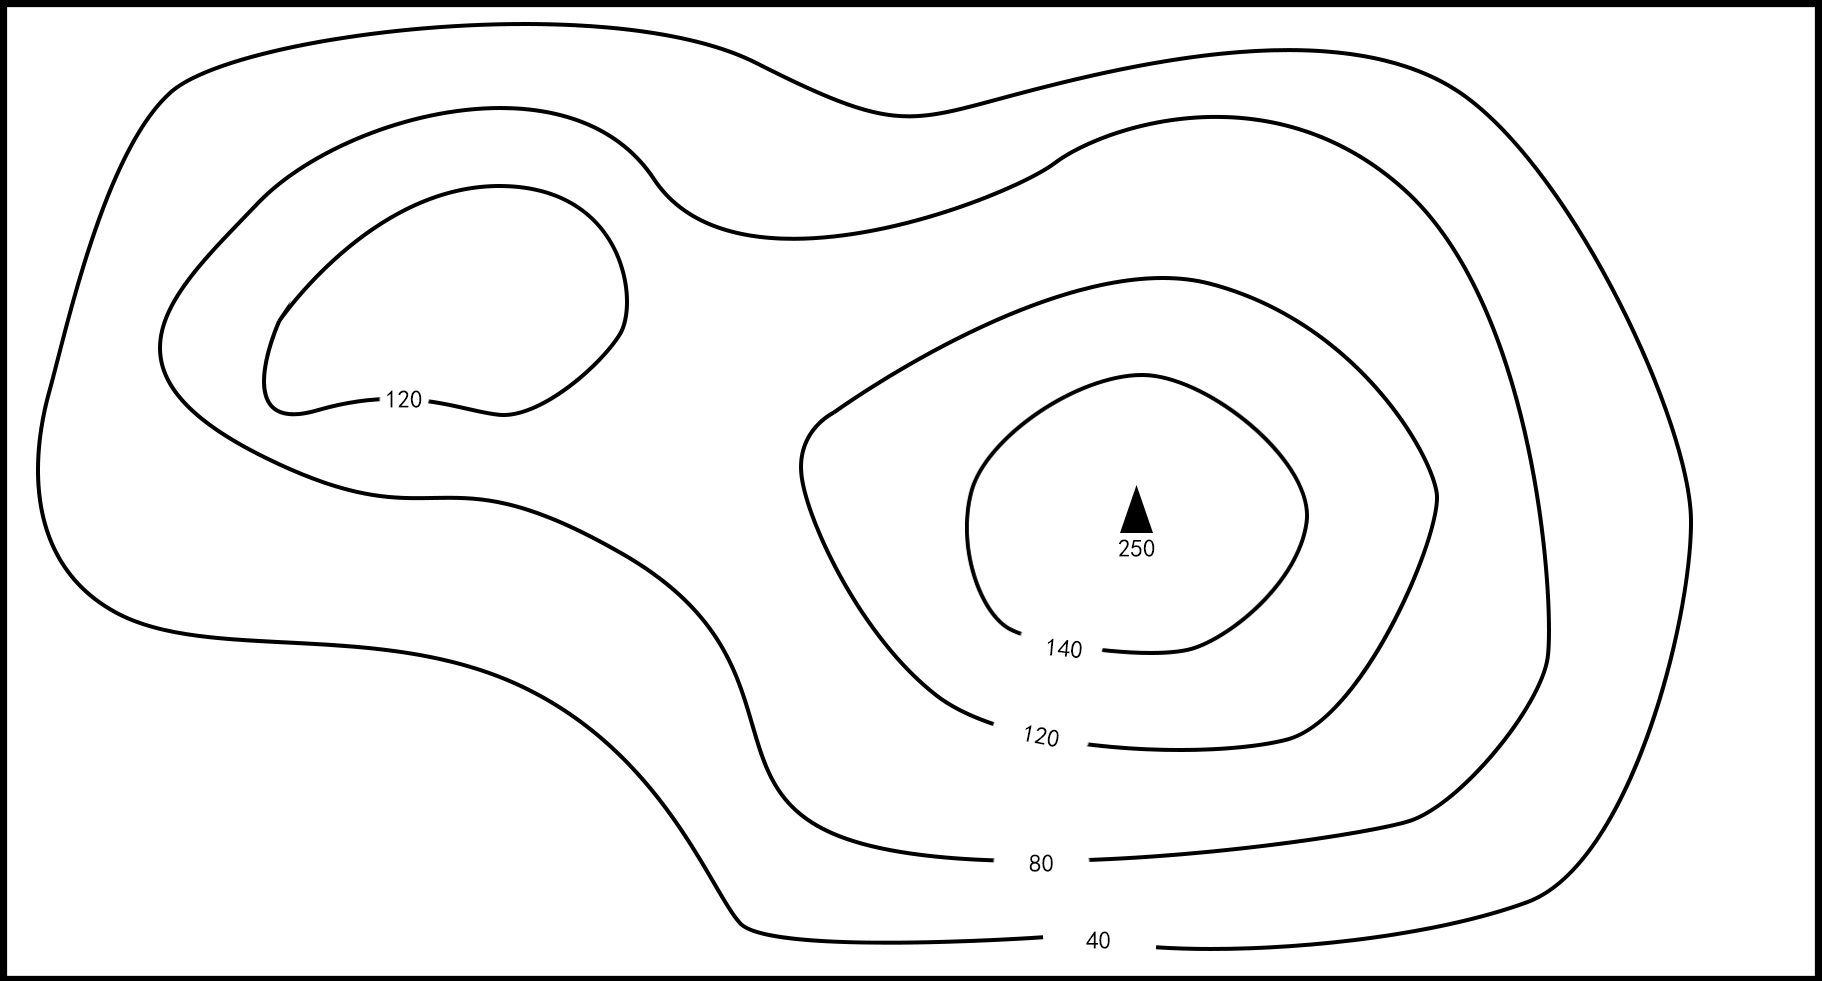
\includegraphics[width=0.75\textwidth]{/map-1/map-1}
  \caption{分层地形图}
  \label{fig:map-1}
\end{figure}

首先进行栅格化。

\begin{algorithm}[h]
  \caption{地图栅格化}\label{algorithm}
  \KwData{原地图 $map$, 地图高度 $L$, 地图宽度 $W$, 栅格大小 $X$}
  \KwResult{栅格化地图 $grid$}
\end{algorithm}

\begin{figure}[h]
  \centering
  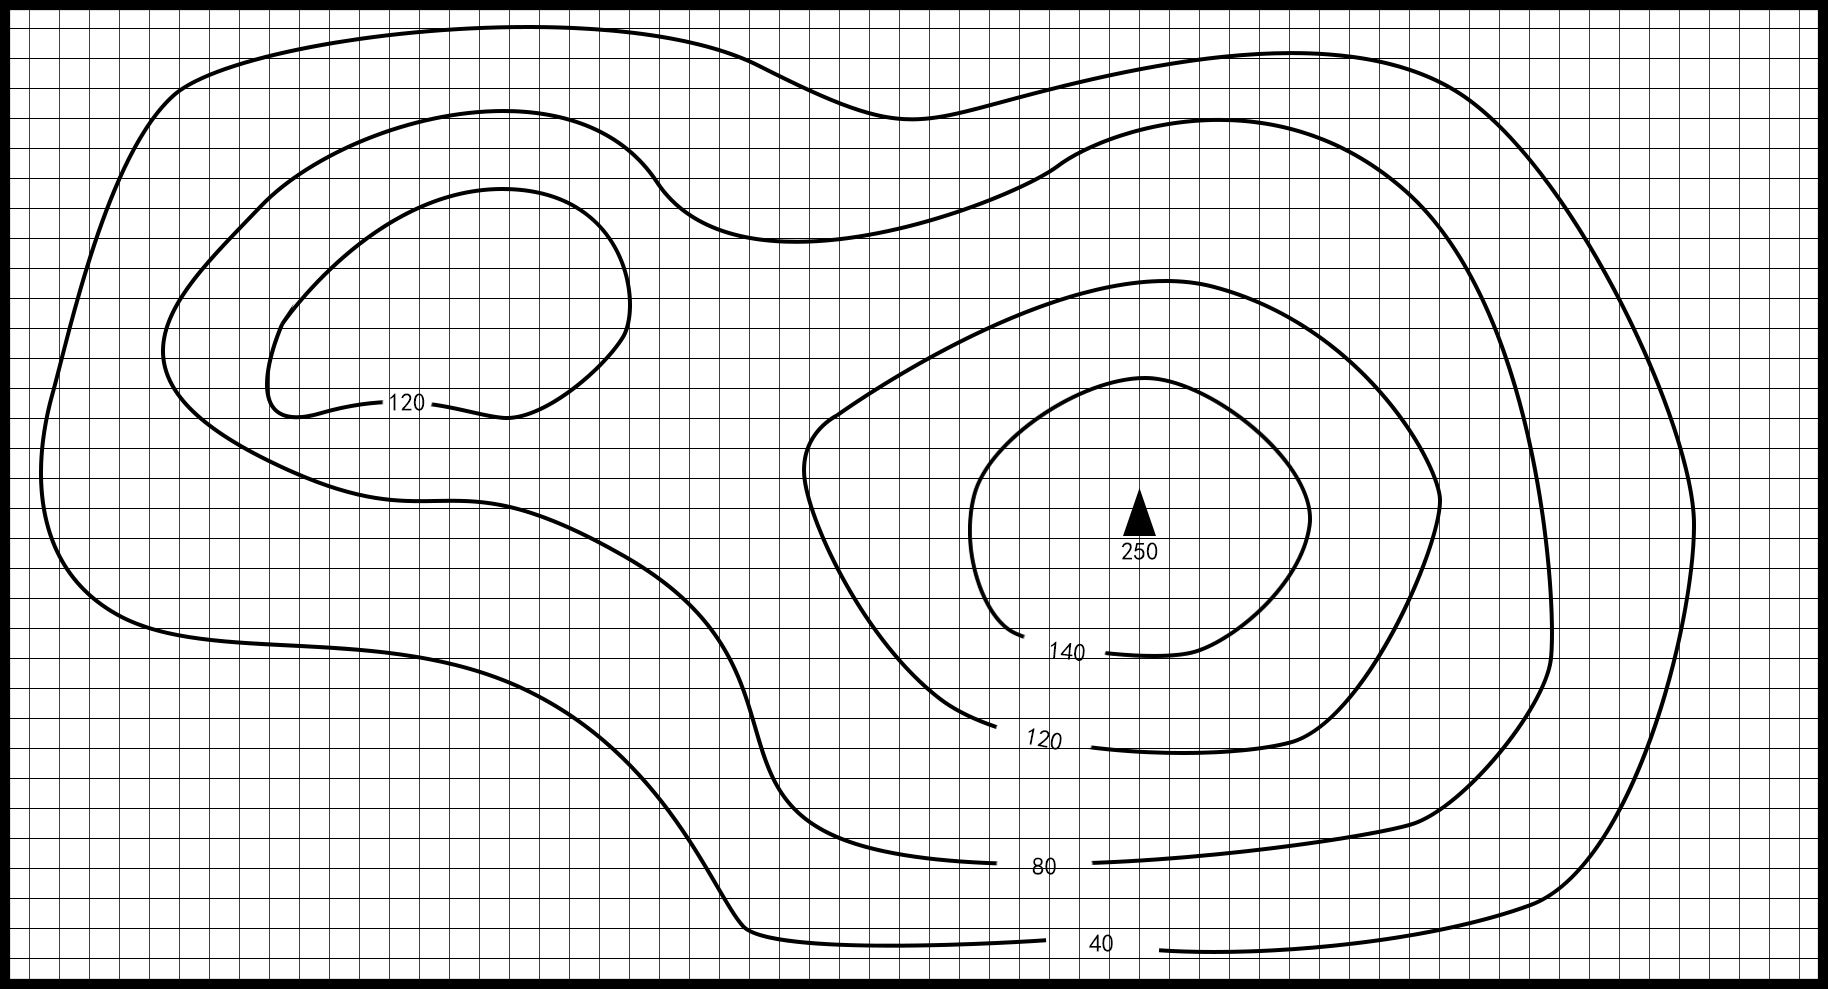
\includegraphics[width=0.75\textwidth]{/map-1/map-1-grid}
  \caption{栅格化后的地图}
  \label{fig:map-1-grid}
\end{figure}

之后以120m高度作为分界,
将栅格地图进行二值化处理:

\begin{algorithm}[H]
  \caption{地图栅格二值化}\label{algorithm}
  \KwData{原栅格地图 $grid$, 界高度$h$}
  \KwResult{二值化栅格化地图 $fin$}
\end{algorithm}

\begin{figure}[H]
  \centering
  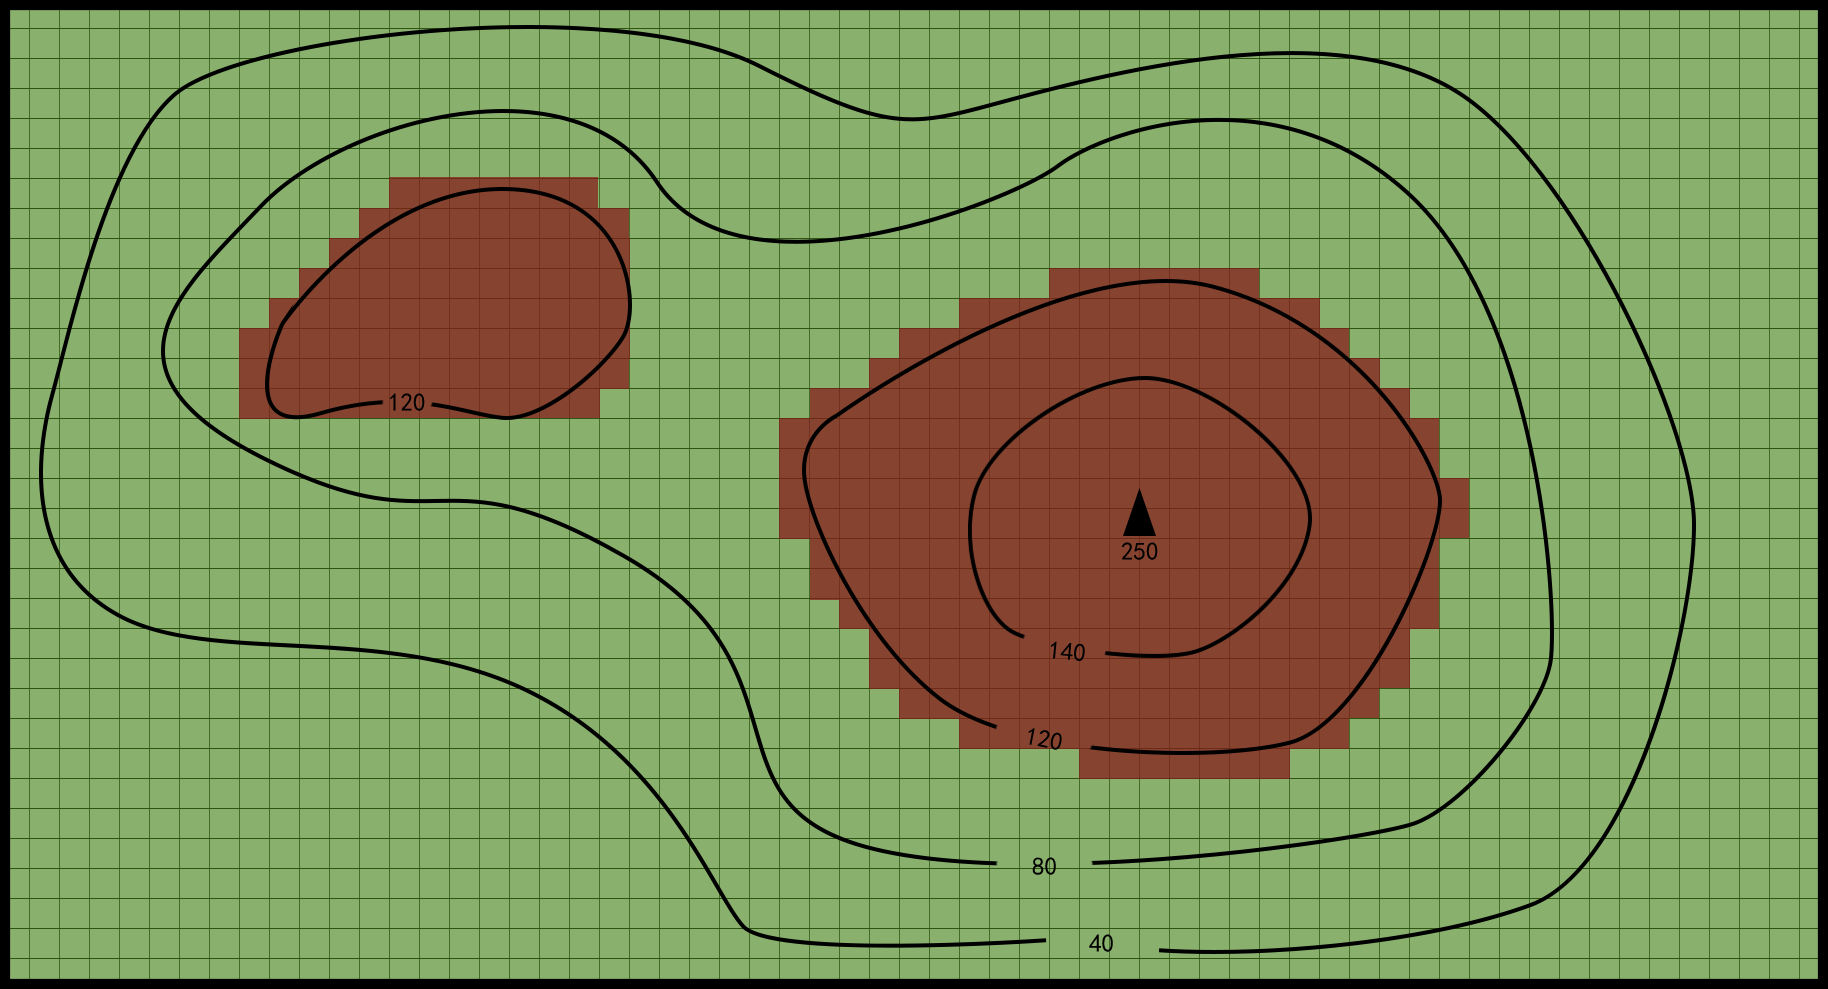
\includegraphics[width=0.75\textwidth]{/map-1/map-1-grid-noted}
  \caption{完成栅格法环境建模的地图}
  \label{fig:map-1-grid-noted}
\end{figure}

这样就完成了航迹图栅格化,即环境空间建模。

%航迹规划算法-------------------------
\newpage\section{航迹规划算法与实现}
\subsection{传统基本航迹规划算法}
\subsubsection{模拟算法}
\subsubsection{Dijkstra单源最短路算法}
\subsubsection{IDA*搜索算法}
\subsection{现代智能航迹规划算法}
\subsubsection{遗传算法}
\subsubsection{蚁群算法(ACA)}
\subsubsection{改进灰狼算法(IGWO)}
\subsubsection{布谷鸟搜索算法(CS)}
%航迹平滑算法-------------------------
\newpage\section{航迹平滑算法}
\subsection{三次样条插值法(Spline 插值)}
\subsection{贝塞尔曲线法(Bézier Curve)}
%航迹平滑算法-------------------------
\newpage\section{结论}
%参考文献库--------------------------------------------------------
\newpage\begin{thebibliography}{20}
\bibitem{ref1}中华人民共和国交通运输部.2024年交通运输行业发展统计公报[R/OL].(2025-06-12)[2025-10-04].https://xxgk.mot.gov.cn/2020/jigou/zhghs/202506/t20250610\_4170228.html.
\bibitem{ref2}欧林联.无人机自动化巡检在城市桥梁运维中的探索和应用[J].福建建设科技,2025,(05):97-100.DOI:CNKI:SUN:FJJK.0.2025-05-024.
\bibitem{ref3}王硕,李洋,赵蕴龙,等.无人机航迹规划算法综述[J/OL].哈尔滨工程大学学报,1-14[2025-10-04].https://link.cnki.net/urlid/23.1390.U.20250616.1544.003.
\end{thebibliography}

\end{document}